\documentclass[letterpaper,11pt]{article}

\usepackage{fullpage,amsmath,amsfonts,latexsym,xcolor,clrscode3e}
\usepackage{graphicx}
\usepackage{amsthm}
\usepackage{hyperref}
\usepackage{fullpage}
\usepackage[ruled,vlined,linesnumbered]{algorithm2e}
\usepackage{enumerate}

\newcommand{\re}{{\mathbb{R}}}
\newcommand\numberthis{\addtocounter{equation}{1}\tag{\theequation}}
\newcommand{\floor}[1]{\lfloor {#1} \rfloor}
\newcommand{\ceil}[1]{\lceil {#1} \rceil}
\newcommand{\paren}[1]{\left( {#1} \right)}
\newenvironment{solution}{\color{black} }{}

\newcommand{\nats}{\mathbb{N}}

\newcommand{\comment}[1]{$\rhd$\ {\small\sf #1}}

\newtheorem{theorem}{Theorem}
\newtheorem{claim}[theorem]{Claim}
\newtheorem{lemma}[theorem]{Lemma}
\newtheorem{problem}{Problem}


\begin{document}
{\noindent\large
{\em Introduction to Analysis of Algorithms} \hfill \today\\
Boston University \hfill CS 330\\
Professor  Adam Smith, Dora Erdos \hfill Fall 2020\\}


\vspace{1pt}
\hrulefill\vspace{3mm}
\begin{center}
{\LARGE\bf Homework 5}\\
{\bf Due Wednesday, October 7 at 11:59 PM}
\end{center}
\begin{center}
    \color{teal}
   Student: Justin DiEmmanuele \\
    Collaborators: Shilpen Patel, George Padavick, Matthew Gilgo
\end{center}



\section*{Homework Guidelines}

\paragraph{Collaboration policy} Collaboration on homework problems, with the exception of
programming assignments and reading quizzes, is permitted, but not encouraged.
If you
choose to collaborate on some problems, you are allowed to discuss
each problem with at most 5 other students currently enrolled in the
class.
Before working with others on a problem, you should think about it
yourself for at least 45 minutes. Finding answers to problems on the
Web or from other outside sources (these include anyone not enrolled
in the class) is strictly forbidden.

{\em You must write up each problem solution by yourself without
assistance, even if you collaborate with others to solve the
problem.} You must also identify your collaborators. If you did not
work with anyone, you should write "Collaborators: none." It is a
violation of this policy to submit a problem solution that you
cannot orally explain to an instructor or TA.

\paragraph{Solution guidelines} For problems that require you to provide an algorithm, you must give the following:
    \begin{enumerate}
\item  a precise description of the algorithm in English and, if helpful, pseudocode,
\item a proof of correctness,
\item an analysis of running time and space.
\end{enumerate}
You may use algorithms from class as subroutines. You may also use any facts that we proved in class.


You should be as clear and concise as possible in your write-up of
solutions. 

A simple, direct analysis is worth more points than a
convoluted one, both because it is simpler and less prone to error and
because it is easier to read and understand. Points might be
subtracted for illegible handwriting and for solutions that are too
long. Incorrect solutions will get from 0 to 30\% of the grade,
depending on how far they are from a working solution. Correct
solutions with possibly minor flaws will get 70 to 100\%, depending on
the flaws and clarity of the write up.

\newpage 
\begin{enumerate}

\item(\textbf{Photography shop})

    Suppose you work at a photography shop, and at the start of your
    workday you are given a list of jobs $i = 1, 2, \ldots, n$, each
    with a processing time $p_i$ and a ``touchiness'' factor $t_i>0$
    (corresponding to how mad the customer will get if job $i$ is
    delayed). Your pay for finishing job $i$ at time $f_i$ is $(P -
    f_i)/t_i$, where $P$ is the total processing time of all jobs ($P
    = p_1 + p_2 + \ldots p_n$).  Assume you have enough time to finish
    all $n$ jobs, but you get to choose the  order in which  you do
    them. You can only do one job at a time.


  The algorithmic problem is to compute an order that maximizes your total payment.
  
  
  For example, suppose you have three jobs as follows:
  
  \begin{center}
\begin{tabular}{ |c|c|c| } 
 \hline
$ i $& $p_i$ & $t_i$ \\ 
 \hline
 1 & 4.5 & 10 \\ 
 \hline
 2 & 1.25 & 7 \\ 
 \hline
 3 & 9 & 3 \\ 
 \hline
\end{tabular}
\end{center}

Then, the order $(1,2,3)$ would have finishing times $f_1 = 4.5$, $f_2 = 5.75$, $f_3 = 14.75$ and a total payoff of $10.25/10 + 9/7 + 0/3 = 2.3$ On the other hand, the ordering $(3,1,2)$ has finishing times $f_3 = 9, f_1 = 13.5, f_2 = 14.75$ with total payoff $5.75/3 + 1.25/10 + 0/7 = 2.04$

  
  
  
  
  

  An idea is to find some quantity by which the tasks can be sorted, so that the optimal
  order is the order sorted by this quantity.
  
  \begin{enumerate}
      \item Consider each of the following orders in which to schedule jobs. For \textbf{three out of the four} of them, give a counterexample showing that it does not produce the optimal task schedule:
      \begin{enumerate}
          \item Decreasing order of processing time $p_i$
          \item Decreasing order of touchiness $t_i$
          \item Increasing order of \emph{product} of touchiness to processing time $t_i p_i$
          \item Increasing order of \emph{sum} of touchiness and processing time $t_i + p_i$
      \end{enumerate}
     \item Give a polynomial-time greedy algorithm for this problem. [An exchange algorithm works well for the proof of correctness.]
  \end{enumerate}

 \emph{Hint}: You may want to analyze the situation
  of two tasks that are scheduled next to each other: say \( (2, 3) \).
  Under what condition on their parameters \( p_{2},t_{2},p_{3},t_{3} \) will be worth changing their
  order to \( (3,2) \)?
  What is the sorting quantity suggested by this condition?
  (Compute the difference in payment resulting from the swap.)
  
  
  \newpage
  \begin{itemize}
      \color{teal}
      \item Part A
  \begin{itemize}
      \item Two of the proposed schedules can be disproved using one example.
           The following example will disprove i and ii. 
          Take the following case in which job i comes before job j in a two
          job set. $p_i = 100$,  $t_i = 100$, $p_j = 1$ and $t_j = 1$ satisfy 
          the following conditions:
          \begin{enumerate}[i]
              \item Decreasing order of processing time as $p_i > p_j$
              \item Decreasing order of touchiness as $t_i > t_j$
          \end{enumerate}
          The dollar amount for ordering $\{i, j\} $ in a schedule with no idle 
          time is represented below:
          \[
              A_{\{i, j\} } = \frac{\left( P - f_i \right) }{t_i} + \frac{\left( P - f_j \right) }{t_j}
          .\] 
          and, 
          \[
          f_i = p_i, f_j = p_i + p_j, P = p_i + p_j
          .\] 
          Which gives:
          \[
              A_{\{i, j\} } = \frac{\left( 101 - 100 \right) }{100} + \frac{\left( 101 - 101 \right) }{1} = 0.01
          .\] 
          If we calculate the reverse order $\{j, i\} $ we get:
          \[
              A_{\{j, j\} } = \frac{\left( 101-1 \right) }{1} + \frac{\left( 101 - 101 \right) }{100} = 100
          .\] 
          Clearly, in this example, it is more advantageous to reverse the order
          to $\{j, i\} $ disproving i and ii.
      \item The last rule, $t_i + p_i < t_j + p_j$ can be disproved with the 
          following example in which $p_i = 5$,  $t_i = 5$, $p_j = 10$, and $t_j = 2$. This set of values complies with rule iv since,
          \[
          5 + 5 = 10 < 10 + 2 = 12
          .\] 
          Following the same procedure as before, the money with each ordering 
          is:
          \[
              A_{\{i, j\} } = \frac{\left( 15 - 5 \right) }{5} + \frac{\left( 15 - 15 \right) }{2} = 2
          .\] 
          \[
              A_{\{j, i\} } = \frac{\left( 15 - 10 \right) }{2} + \frac{\left( 15 -15 \right) }{5} = 2.5
          .\] 
          The reverse ordering gives a better payout so iv is disproved.

  \end{itemize}

  \newpage
  \item Part B
      \begin{itemize}
          \item A precise definition of the algorithm in English and, if helpful, pseudocode.

              \begin{itemize}
                  \item The algorithm takes in an array $p$ with processing time
                      $p_i$ for jobs $i = 1, \ldots, n$ and an array $t$ with 
                      touchiness scores for jobs of the same index. 
                      $O\left( 1 \right) $ time.
                  \item We initialize an array $O$ that contains the index values
                      $i = 1, \ldots, n$ to keep track of where each job is 
                      swapped to. $O\left( 1 \right) $ time.
                  \item Initialize an empty array $prod$ that is used to hold
                      the products of jobs $i = 1, \ldots, n$. $O\left( 1 \right) $
                      time.
                  \item We iterate through both $p$ and $t$ at once and store 
                      their product in the corresponding index of $prod$.
                      $O\left( n \right) $ time.
                  \item Use merge sort to iterate through
                      $prod$ and swap any two values in which the previous 
                      index is greater than the index adjacent to it. Any time 
                      an index is switched in $prod$, switch the indexes in  $O$.
                      $O\left( n\log{n}\right) $ time.
                  \item Return $O$ which contains the ordering of the optimal 
                      set of jobs. $O\left( 1 \right) $
              \end{itemize}

          \item A proof of correctness. \\

              Take a set of jobs $S = \{0, \ldots, n\} $ where job $i$ has a
              process time $p_i$ and touchiness factor $t_i$. There are two jobs
              $a$ and $b$ that are adjacent to each other with $b > a$. Since 
              swapping two jobs has no impact on the rest of the jobs' start 
              and finish times, we can analyze what happens to the payout 
              if these jobs are switched. \\


              We define the following variables: $s$ is the start time of the 
              first job in the pair - this does not change regardless of order.
              $f$ is the finish time of the pair of jobs - this also does not 
              change and is equal to $p_a + p_b$.\\

              If we assume that amount $A_{\{a, b\} }$ is greater than $A_{\{b, a\} }$, we see that it implies the following:
              \[
                  A_{\{a, b\} } = \frac{\left( P - s - p_a \right) }{t_a} + \frac{\left( P - s - p_a - p_b \right) }{t_b} > \frac{\left( P - s - p_b \right) }{t_b} + \frac{\left( P - s - p_a - p_b \right) }{t_b} = A_{\{b, a\} }
              .\] 
              Which simplifies to:
              \[
              p_at_a < p_bt_b
              .\] 
              Which turns out to be the rule! This shows that for any pair of 
              adjacent jobs, choosing the smaller product $p_it_i$ will increase 
              the payout.\\

              \begin{itemize}
                  \item It is clear that an optimal schedule will have no idle 
                      time as delaying a job needlessly will only decrease its
                      payout ($f_i$ increases).
                  \item All schedules with no inversions as defined by rule iii
                      given in the problem statement have the same pay out.
                      Any jobs that are in a different order in two job orderings 
                      must have the same payout per the algebraic simplification 
                      above. (If we assume equal instead of greater than we see
                      that $p_at_a = p_bt_b$)
                  \item There exists a job ordering with no inversions and no idle
                      time that is optimal. If there are two jobs $i$ and $j$ 
                      where $p_it_i > p_jt_j$ we know we can swap them and 
                      increase the payout. The job set will have 1 less inversion.
                      Any job set will have a maximum $n \choose 2$ inversions.
                  \item Since lowering the number of inversions only increases 
                      the payout and our algorithm gives the least number of 
                      inversions (none). Our algorithm is optimal.
              \end{itemize}

          \item An analysis of running time and space.
              \begin{itemize}
                  \item Time Complexity\\
                      The algorithm has time complexity of the steps associated
                      above. The most time-intensive step is the sorting of the 
                      arrays done in $O\left( n\log{n}\right) $ time. 
                  \item Space Complexity\\
                      The most space consuming data structure used is the size
                      of the input which is simply $O\left( n \right) $
              \end{itemize}
      \end{itemize}
  \end{itemize}
  
  
  
  
  
  \newpage
  \item(\textbf{Cell towers}) Suppose you are back on the long country road from Lab 3, which we can think of as a line segment with western and eastern endpoints. Let's identify points on the road with the interval $[0,1)$. Now, suppose that a  telecommunications company has invested in cell coverage for this road: they've placed $n$ towers, each of which can cover a different radius  in specific locations along this road such that every segment of the road is covered by \emph{at least} one tower. We'll say $t_i\in [0,1)$ is the location of the $i$-th tower along the road, and it has radius $r_i$. For technical reasons, tower $i$'s interval of coverage will be open on the right side, giving $[t_i - r_i, t_i + r_i)$. 
  
  As a surveyor for this telecommunications company, your job is to find the \textit{maximum size set of points along the road $[0,1)$ such that each
tower serves at most one point in this set}; we'll call a  set with this property \textit{sparse}.  The input for this problem is the list of pairs $(t_i,r_i)$, for $i=1,...,n$.



Below is an example of a set of towers and orange lines indicating a sparse set. (Do not hand in) Is it the largest possible sparse set?

\begin{center}
    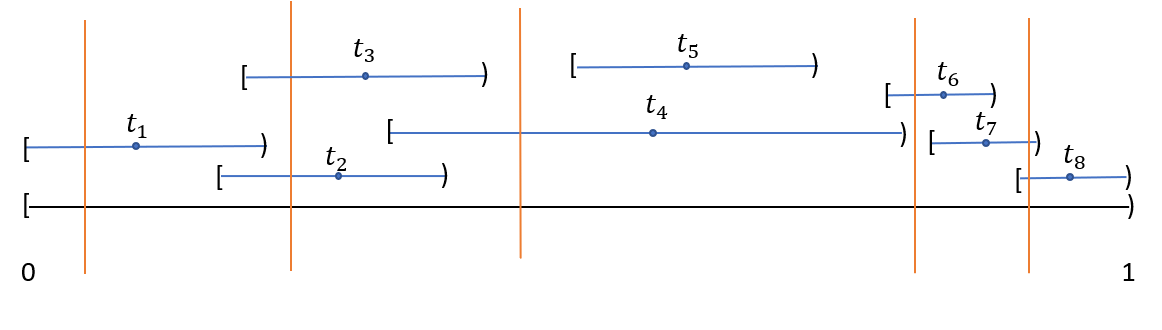
\includegraphics[scale=0.7]{cell_tower_set}
\end{center}



\newpage
\begin{enumerate}
    \item Your friend suggests the following greedy approach: sort the intervals according to their centers $t_i$. Moving from left to right, add $t_i$ (the position of tower $i$) to your set as long it it doesn't conflict with the previous ones (meaning no interval covers both $t_i$ and a previously selected center). Give an example showing why this will not produce the largest sparse set. [NB: this algorithm chooses tower locations, but a sparse set doesn't have to be limited to tower locations—any subset of $[0,1)$ is ok.]
\end{enumerate}

\begin{itemize}
    \color{teal}
    \item The image below displays the algorithm described in a in red on the 
        provided example. An example of a larger sparse set is given in green 
        as a counter example.
        \begin{figure}[htpb]
            \centering
            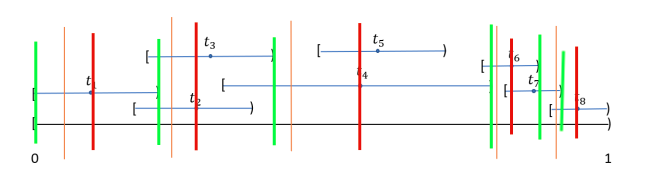
\includegraphics[width=0.8\textwidth]{2a}
            \caption{2.a Counterexample in Red}
            \label{fig:2a}
        \end{figure}

        Clearly, the green set shows a larger sparse set, so the approach
        suggested in red is not optimal.
\end{itemize}


Before we design an algorithm for finding sparse sets, let's consider a related problem: as before, you are again given the fixed locations and radii of $n$ towers, but now suppose that the telecommunications company has decided that, in the interest of profits, they only want to keep enough cell towers running so that every point on the road $[0, 1)$ is covered by at least one tower. We will call such a set of towers \textit{sufficient}. It's now your job to tell them the \emph{minimum} number of towers they need to power so that the whole $[0,1)$ interval is covered (i.e. find a sufficient set of minimum size).

(Do not hand in) How small a set of sufficient intervals can you find for the example pictured above?


\begin{enumerate}
    \item[(b)] Prove that if there exists a sparse set $\mathcal{P}$ of locations with $\lvert\mathcal{P}\rvert = k$, 
    we  need at least $k$ towers to cover $[0,1)$ (that is, every sufficient set $\mathcal{T}$ of towers satisfies $\lvert \mathcal{T}\rvert \geq k$).
    \begin{itemize}
        \color{teal}
        \item We know that set $\mathcal{T}$ is a sufficient set of towers and 
            $\mathcal{P}$ is a sparse set
        \item If we assume $\lvert \mathcal{T}\rvert < k$: we know that in a 
            sparse set each tower can only serve one point in $\mathcal{P}$ 
            so we can assign one tower to each location in $\mathcal{P}$. We 
            run into an issue because there are not enough towers to cover
            each point without a tower serving two points.
        \item Therefore, by contradiction, every sufficient set of 
            $\mathcal{T}$ of towers must satisfy 
            $\lvert \mathcal{T}\rvert \geq k$).

            \newpage
    \end{itemize}
    \item[(c)] Give a polynomial-time algorithm that takes as input a list of pairs $(t_i,r_i)$ and produces both a sparse set of positions  and a sufficient set of intervals, such that the two sets have the same size. (Remember to follow the usual guidelines for algorithms.)
        \begin{itemize}
    \color{teal}
            \item The algorithm is described below:


\begin{algorithm}[H]
      \caption{test($A$)} 
      \KwIn{List $T$ of pairs of $(t_i, r_i)$ for each tower $i$}
      $L$; initialize list to hold left bound of tower $i$ \;
      $R$; initialize list to hold right bound of tower $i$ \;
      $I $; initialize list to hold set of sufficient tower intervals \;
      $P$ ; initialize list to hold set of sparse points \;
      $CurrentMax = 0$; initialize variable to track the current known right most interval that encompasses previous point \;
      $CurrentTower$; initialize variable to track the current known best tower choice \;
      $IntervalMin$ = 0; Initialize minimum of interval\;
      $IntervalMax$ = 1; Initialize max of interval\;
      \For{$i = 0$ to $T.length\left( \  \right) - 1 $ }{
          $L[i] = T[i][0] - t[i][1]$ \;
          $R[i] = T[i][0] + t[i][1]$ \;
      }
      \While{$CurrentMax < IntervalMax$}{
          \For{$i = 0$ to  $T.length$} {
              \If{$LastPoint \ge  L[i]$}{
                  \If{$R[i] > CurrentMax$ }{
                      $CurrentMax = R[i]$\;
                      $CurrentTower = i$\;
                  }
              }
          }
          $LastPoint = CurrentMax$
          $I.append(CurrentTower)$\;
          \If{$CurrentMax \neq IntervalMax$}{
              $P.append(CurrentMax)$\;
          }
      }
      \KwOut{$I, P$}
\end{algorithm}

    The idea of this algorithm is to start by putting a point in the sparse set
    at the start of the interval since we know there is a sufficient set of 
    towers. We then chose the tower that both covers this point and reaches 
    the furthest towards the end of the interval. We then place 
    the next point directly at the end of that tower and repeat until
    we have reached the end of the interval.\\

    This algorithm, in effect, greedily chooses the tower that reaches furthest
    Towards the end that also includes the previous chosen point.

\item Proof of correctness\\

    We will prove this algorithm by contradiction. The algorithm claims to find
    a sparse set of points and a sufficient set of intervals. To test this, let
    us assume we find a set of points $\{a, b\} $ that are covered by the same
    tower.\\

    If $a$ is placed into a sparse set the algorithm will then check for the 
    tower that reaches the farthest to the right in which $a$ falls under it.
    Another point is only added AFTER this interval it decides on. This makes
    it impossible for $a$ and $b$ to be placed in the same sparse set.\\

    Similarly we can assume that we find a sparse set in which the number of 
    towers is not equal to the number of points in the set. For this to happen
    a point must be added to the set that already has a corresponding tower
    that covers it. This is impossible because the algorithm only adds points 
    directly AFTER every added tower. \\

\item Time Complexity\\
    This algorithm must iterate through all $n$ towers in the inner for loop. 
    The question is - how many times does that inner for loop block get run?
    Since towers are only added in increasing reach to the right of the interval
    and there are only $n$ towers, the outer while loop will run a maximum of 
    $n$ times. This makes the time complexity $O\left( n*n \right) = O\left( n^2 \right) $.



        \end{itemize}
    
        \newpage
    \item [(d)] Argue that the algorithm from (c) finds both a sparse set of maximum possible size, and a sufficient set of the smallest possible size. 
        \color{teal}

        We will prove d using the greedy stays ahead approach. For finding the 
        sufficient set of towers, the greedy rule we use is essentially - 
        chose the next tower that has an overlapping interval (so there are no
        gaps) and that reaches as far right as possible. We want to prove that 
        in an optimal algorithm the tower $i$'s corresponding tower in our 
        algorithm's covers at least as far to the right of the interval. \\

        For towers $0, \ldots, n$ in our solution, $t_i + r_i$ is at least as 
        large or larger. This is obviously true for the base case where the 
        interval starts at zero, since the algorithm chooses the interval with
        the furthest range to the right. At this point we know our algorithm 
        reaches at least as far as the optimal solution. We assume this is true
        up to tower $n - 1$. At step  $n$ the greedy algorithm chooses the step 
        furthest to right once again. By induction, the algorithm must find 
        the smallest sufficient set as it will reach the end of the interval
        in the shortest number of steps.\\

        Similarly we can then prove maximum sparse set size. The points in the 
        sparse set are added as soon as the previous interval that covered the 
        previous point ends. Whenever it is possible to place another point 
        into he 
\end{enumerate}
  

\end{enumerate}
\end{document}
